\documentclass[10pt, headsepline,DIV14,BCOR0.5cm]{scrreprt}
\usepackage[utf8x]{inputenc}
\usepackage[T1]{fontenc}
\usepackage{arev}
\usepackage{booktabs}
\usepackage{parskip}
\usepackage{setspace} 
\usepackage{multicol}
\usepackage{natbib}
\usepackage{hyperref}
\usepackage{graphicx}

\setlength{\parindent}{0cm}
\setlength{\parskip}{2em}
%\linespread{1.3}


\hypersetup{pdfborder=0 0 0, colorlinks=true, linkcolor=black, anchorcolor=black, citecolor=black, urlcolor=blue}


% Title Page
\title{TRiCYCLE Users Manual}
\author{Peter Brewer, Daniel Murphy and Esther Jansma}
\publishers{\footnotesize{Cornell University, Ithaca, New York \\ Cultural Heritage Agency (RCE/OCW), Amersfoort, The Netherlands }}
\date{Version 0.2}


\usepackage{mdwlist}

\begin{document}
\maketitle


\tableofcontents

\chapter{Acknowledgements}

Funding for the development of TRiCYCLE has been provided by NWO section Humanities through the
DCCD project and through the various patrons of the Malcolm and Carolyn Wiener Laboratory for Aegean
and Near Eastern Dendrochronology.

We would like to thank the numerous contributors to the open source libraries used by TRiCYCLE and
its associated libraries. We would also like to thank Lars-Åke Larsson, Rémi Brageu, Pascale Fraiture,
Henri Grissino-Mayer, Patrick Hoffsummer, Bernhard Knibbe, George Lambert, Catherine Lavier, Hubert
Leuschner, Martin Munro, Ian Tyers and Ronald Visser for assistance understanding many of the data
formats implemented.

\chapter{What is TRiCYCLE?}

TRiCYCLE is a universal dendrochronology file format converter. It currently has support for reading and
writing 18 different file formats:

\begin{table*}[htbp]
\label{tbl:supportedFormats}
\caption{Formats supported by TRiCYCLE}
\begin{center}
\begin{tabular*}{10cm}{ l @{\extracolsep{\fill}} c  c }
  \toprule
 Format & Read support & Write support\\
 \midrule

Belfast Apple      	 & \checkmark  & \checkmark \\
Belfast Archive   	 & \checkmark  &            \\
Besan\c{c}on		 & \checkmark  & \checkmark \\
CATRAS			 & \checkmark  &            \\
Comma Separated Values	 &             & \checkmark \\
Corina Legacy		 & \checkmark  & \checkmark \\
Excel			 &             & \checkmark \\
Heidelberg		 & \checkmark  & \checkmark \\
Nottingham		 & \checkmark  & \checkmark \\
PAST4			 & \checkmark  & \checkmark \\
Sheffield		 & \checkmark  & \checkmark \\
Topham			 & \checkmark  & \checkmark \\
TRiDaS			 & \checkmark  & \checkmark \\
Tucson			 & \checkmark  & \checkmark \\
Tucson Compact		 & \checkmark  & \checkmark \\
VFormat			 & \checkmark  & \checkmark \\
WinDENDRO		 & \checkmark  &            \\

\bottomrule
\end{tabular*}
\end{center}
\end{table*}


TRiCYCLE extracts both data and any metadata present in files and converts them to the Tree-Ring Data
Standard (TRiDaS) data model. As TRiDaS is capable of representing the full range of dendro data and
metadata, it is then possible to write out the file to any one of the supported formats.
Key features of TRiCYCLE are:

\begin{itemize*}
 \item Seamless support for units where possible
 \item Interpretation of all metadata
 \item Handling of different charactersets and line feeds from different operating systems
 \item Comprehensive warning and exception system which provides detailed feedback when errors are
detected in files
\end{itemize*}


For a complete discussion of TRiCYCLE and its underlying libraries please see \citep{tricycle}.


\chapter{Installation}

TRiCYCLE is a Java application and so can be installed on any modern operating system. To make
installation more familiar though we have packaged it up into native installers for Windows, Mac OSX
and Linux. Download the relevant package for your operating system from the SourceForge \url{http://
tridas.sf.net} website.

\begin{description}
 \item[Windows] - Run the setup program and follow the steps. The program will be installed to your hard disk
and shortcuts added to your start menu. If you do not have Java installed on your system or
you do not have the required version the installer will provide you with assistance to do so.
 \item[Mac OSX] - Open the .dmg file in Finder. Drag the TRiCYCLE.app file into your Applications folder, or
wherever you'd like it installed. MacOSX comes pre-installed with Java so there is no need
to install it separately.
 \item[Linux] - An Ubuntu deb package is provided for TRiCYCLE. Install this package with your standard
package manager (e.g. sudo dpkg --install TRiCYCLE\_X.X.deb). It includes information
on the required dependencies therefore it should install everything you need if you are
running Ubuntu. On other distributions you may find that the dependencies do not install
automatically and the TRiCYCLE installation fails. If this is the case you will have to install
sun-java6-jre first manually.
\end{description}


\chapter{How to use TRiCYCLE}

The first step is to specify the format of your input file(s). Choose your input file format from the pull
down list on the File List page. Then you need to specifiy the file(s) that you would like to convert. This
can be done in a variety of ways:

\begin{itemize*}
 \item Click the browse button
 \item Use the \verb|File > Open| menu
 \item Drag files onto the dialog box from your file manager (e.g. Finder on MacOSX, My Computer on
Windows or Nautilus, Dolphin, Konqueror etc on Linux).
\end{itemize*}

Once you have your list of files prepared you can then go to the Convert tab.


On the Convert page, the next thing you need to do is select the desired output format from the drop down
list. Next, press the convert button and after a short delay your files should appear in the list below. At the
bottom of the window, you'll see a summary showing how many files were processed, how many of the
convertions failed and how many were converted successfully but with warnings.


The results of the conversion are shown in a tree view on the convert tab. Files that failed to convert are
highlighted by a red cross along with a message explaining what went wrong. Each file that converted
successfully and with no warnings is shown with a green tick icon below which are shown the output file
or files. Depending on the input and output formats chosen, a input file may be converted into one or more
output files as some formats can store just one series while others can store multiple series.


\begin{figure}
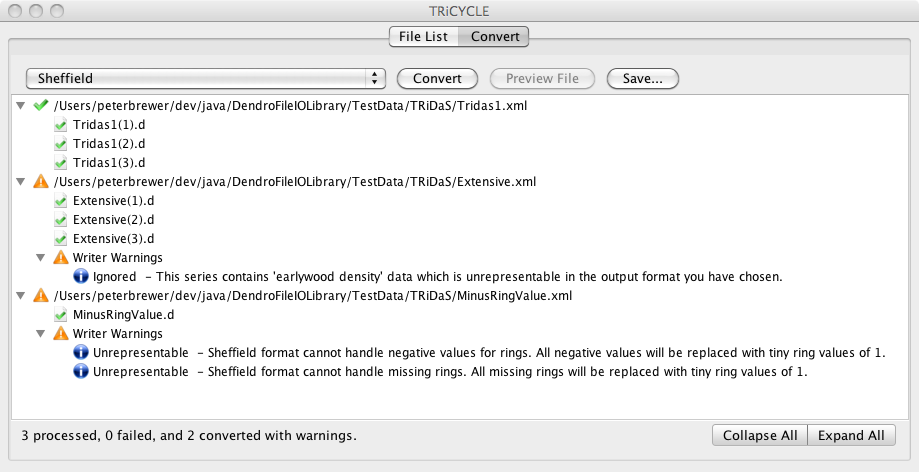
\includegraphics[width=\textwidth]{screenshot1.png}
\caption{Screenshot showing the conversion of three TRiDaS files into Sheffield
format. The second and third files both include warnings that the Sheffield format
is unable to fully represent all the data in the input files.} 
\label{fig:screenshot}
\end{figure}

If there were warnings produced during the conversion process, then the file will be marked with a orange
exclamation icon. Warnings can be associated with either the process of reading the input file, or writing
the output file. They can also be related to a single series within the file or the input file as a whole. The
warning messages are displayed to illustrate the context of the warning. Longer warnings will scroll of the
edge of the window, but if you hover your mouse over the warning a tooltip will show the entire message.

If you would like to preview the result of the conversion process you can double click on the output files
and they will be displayed in a text viewer. This option is not, however, available for binary formats such
as CATRAS and Excel.

Once you are happy with the results of the conversion you can save the files permanently to disk by pressing
the save button. It will offer you the option of specifying which folder to save the files to.


\chapter{Options}

The options panel is available from the file menu. It is split into two sections: Reader config and Writer
config.

\section{Character sets}

The character set can be set for both the file being read and the file being written. The character set is
the system for pairing computer character codes with the character glyphes that we read. The widely
used standard was originally ASCII, but this does not include diacritic characters, and characters specific
to certain languages. There have since been many character encodings proposed (e.g ISO 8859-1 for
Western Europe and ISO 8859-7 for Greece) as well as some that are specific to Windows and Mac
operating systems (e.g. Windows-1252 and MacRoman). The character set that is becoming most widely
used is Unicode UTF-8. This is capable of representing all 107,000+ distinct characters while remaining
backwards compatible with ASCII for the 128 characters that it is able to represent.

If an incorrect character encoding is used to interpret a file, normally the majority of characters will display
correctly (where the character sets share the same encodings) but more unusual characters will be displayed
incorrectly - typically square boxes or question marks.

TRiCYCLE can using the NIO package to attempt to automatically detect which encoding a file is in.
Unfortunately, there is no full-proof way to do this, so by default, this feature is turned off. If you are
having problems with character encodings you may like to choose 'Automatic' in the charset box if you
have no idea what character encoding your file is in.

The character encoding is set to the default for the operating system you are running. For instance on
MacOSX this will be MacRoman and for Windows it will be Windows-1250. If you know your input file
is in a different encoding you should set it in the input charset box. If your output file needs to be read
on an operating system other than the one you are currently running, then you may like to override the
writer charset. Please note that for certain writers, the character set used is part of the file specification
(e.g. TRiDaS must be UTF-8). In this case your choice will be ignored.

The final complication with regards character sets is the line feed character(s). For historical reasons
different operating systems use different characters to represent a new line. Depending on the software
that is used to read a file, this can cause problems. TRiCYCLE itself will automatically adapt to files with
any type of line feed characters so reading files in TRiCYCLE will never be a problem. When writing
out files, TRiCYCLE will use the default line feed for the operating system you are running, unless you
choose a platform specific character set. For instance if you run TRiCYCLE on Windows and choose a
MacRoman writing charset, TRiCYCLE will use Mac style line feeds.


\section{Metadata editor}

TRiCYCLE works by reading in a data file and translating it into the TRiDaS data model. TRiDaS has
a rich array of fields to represent all manner of dendro data and metadata. Although most of these are
optional, the TRiDaS specification requires that a handful of these are always filled in. Unfortunately many
of the legacy data formats do not contain information for these mandatory fields, therefore TRiCYCLE
must fill these with default values. You will most commonly see these defaults as 'Unnamed object' etc in
your output file. The metadata editor enables you to override these default values.

Clicking on the reader metadata editor button in the options window will give a table of all the metadata
fields that will be set automatically by TRiCYCLE along with their current values. You can change most
of these with the exception of those that are required to be a controlled vocabulary. These will require a 
more complicated interface which we haven't had time to implement yet. The third column in the editor is
a tick box to specify whether the value is overriding or not. If ticked, the value specified in this editor will
be used regardless of whether a value can be extracted by TRiCYCLE from the input datafiles.

An identical editor is available for the writer. These are the default values used by the writer code for
your chosen output format. For instance, TRiDaS does not require that a start year field be set (as in the
case of relatively dated series), whereas some output formats do require such a field. If an input file does
not contain start year information then some writers need to know which default value for start year to
use. Like for the input metadata editor, you can set fields to `overriding' which means they will be used
regardless of whether this information is available in the input dataset.

\section{Naming convention}

Some file formats can contain just one data series while others can contain many. When converting from
a multi-series format to a single series format this means that one input file is converted to multiple output
files. The naming convention is used to determine how to name the output files. The naming convention
relates to the filename itself and not the file extension. The file extension is specific to the output format
chosen (e.g. Heidelberg files are .fh and TRiDaS files are .xml).

\begin{description}
 \item[Numerical] - This is the default naming convention. It uses the name of the input data file and
appends an incrementing number if more than one output file is produced.
 \item[UUID] - This gives all output files a random named based on Universally Unique Identifiers
(UUIDs). This is a 36 character hexidecimal code which due to the astronomically
large number of possible combinations is guaranteed to be universally unique. A
typical filename will look like: 550e8400-e29b-41d4-a716-446655440000.
 \item[Hierarchical] - This uses the hierarchical structure of the TRiDaS data model to provide a meaningful
name for the output file. It joins together the title of each entity in the file beginning
with the project name through to the series name. For files that contain multiple series,
the name will contain details of all the entities shared by all the series in the file. For
example, if a file contains several series from the same sample, then the file name
will be projectTitle-objectTitle-elementTitle-sampleTitle. If the file contains several
series from different samples of the same object, then the file would be projectTitle-
objectTitle. If multiple output files end up with the same name then like the numerical
convention described above, the files will have an incremental number appended to
the end. Unfortunately, most input data files do not contain rich name information
so files end up being called unnamedProject-unnamedObject-unnamedElement etc.
This convention is therefore more appropriate when converting from TRiDaS to other
formats.
 \end{description}


\chapter{Help and more information}

The best place to start is through the TRiDaS website (\url{http://www.tridas.org}) and the
Dendro Data Standards forum. The forum is a email list for the discussion of TRiDaS and other dendro
data standards issues. It is open for all to join by emailing Peter Brewer (\href{mailto:p.brewer@cornell.edu}{p.brewer@cornell.edu}).

TRiCYCLE is an open source product therefore we are very pleased to welcome anyone that would
like to assist in its development. This obviously includes programmers, but also people willing to help
with documentation and translations too. To find out more information please contact Peter Brewer
(\href{mailto:p.brewer@cornell.edu}{p.brewer@cornell.edu}).

\part*{Appendix - File format descriptions}

\appendix
\chapter{Belfast Apple}

\begin{table*}[htbp]
\label{summary:belfastApple}
\begin{center}
\begin{tabular*}{15cm}{ l @{\extracolsep{\fill}} p{9cm} }
  \toprule

Format name     	 & Belfast Apple \\
Other name(s)      	 & None known \\
Type      	 	 & Text file \\
Extension(s)      	 & Various (typically txt and dat) \\
Read/write support     	 & Read and write \\
Reference implementation & No original software is known to exist so TRiCYCLE is proposed as the reference implementation \\
Data / metadata      	 & Data only with comment \\
Calendar type		 & n/a \\
Absolute dating support	 & No \\
Undated series support   & Yes \\
Relative dating support  & No \\
Multi series support	 & No \\
Original designer	 & John Pilcher \\

\bottomrule
\end{tabular*}
\end{center}
\end{table*}


\section{Description}
Belfast Apple is a simple text file format (see also Belfast Archive [/corina-manual/Belfast Archive])
originating from the Queens University Belfast lab and originally designed for use on an Apple II computer.
This format is not known to be actively used but a large amount of data (especially at Belfast) is archived
in this format.

\begin{itemize*}
 \item Line one contains the name of the site or object the data refers to.
 \item Line two contains the identifier for the sample the data refers to.
 \item Line three contains the number of data values in the file
 \item Lines four onwards contain line feed delimited data values as integers in 1/100th mm
 \item Final line contains a comment typically starting with 'COMMENT -'
\end{itemize*}



\chapter{Belfast Archive}

\begin{table*}[htbp]
\label{summary:belfastArchive}
\begin{center}
\begin{tabular*}{15cm}{ l @{\extracolsep{\fill}} p{9cm} }
  \toprule

Format name     	 & Belfast Archive\\
Other name(s)      	 & None known\\
Type      	 	 & Text file\\
Extension(s)      	 & Various (typically arx, txt and dat)\\
Read/write support     	 & Read only\\
Reference implementation & No original software is known to exist so TRiCYCLE is proposed as the reference implementation\\
Data / metadata      	 & Data with limited metadata\\
Calendar type		 & Gregorian\\
Absolute dating support	 & Yes \\
Undated series support   & No \\
Relative dating support  & No \\
Multi series support	 & Yes \\
Original designer	 & Martin Munro\\

\bottomrule
\end{tabular*}
\end{center}
\end{table*}

\section{Description}

Belfast Archive is a simple text file format based on the original Belfast Apple format at the Queens University Belfast lab. It shares the same features as Belfast Apple but with the addition of a number of metadata fields at the end of the file.

\begin{itemize*}
    \item  Line 1 contains the name of the site or object the data refers to.
    \item  Line 2 contains the identifier for the sample the data refers to.
    \item  Line 3 contains the number of data values in the file
    \item  Line 4 onwards contain line-feed delimited data values as integers
    \item  The lines \verb|"[[ARCHIVE]]"| and \verb|"[[ END OF TEXT ]]"| denote the start and finish of the metadata section  
\end{itemize*}

The metadata section contains the following lines:

\begin{itemize*}
    \item  Line 1 - start year as an integer.
    \item  Line 2 - unknown
    \item  Line 3 - Double representing the resolution of data values e.g. .1= 1/10ths mm, .01 = 1/100th mm, .001 = microns etc
    \item  Line 4 - unknown
    \item  Line 5 - unknown
    \item  Line 6 - unknown
    \item  Line 7 - Title of the data series
    \item  Line 8 - unknown
    \item  Line 9 - unknown 
\end{itemize*}

\chapter{Besan\c{c}on}

\begin{table*}[htbp]
\label{summary:besancon}
\begin{center}
\begin{tabular*}{15cm}{ l @{\extracolsep{\fill}} p{9cm} }
  \toprule

Format name     	 & Besan\c{c}on \\
Other name(s)      	 & SYLPHE\\
Type      	 	 & Text file\\
Extension(s)      	 & txt\\
Read/write support     	 & Read and write\\
Reference implementation & \\
Data / metadata      	 & Data and some structured metadata\\
Calendar type		 & Gregorian\\
Absolute dating support	 & Yes\\
Undated series support   & Yes\\
Relative dating support  & No \\
Multi series support	 & Yes \\
Original designer	 & Georges Lambert\\

\bottomrule
\end{tabular*}
\end{center}
\end{table*}

\section{Description}

The Besancon format is most commonly used in a number of French laboratories. The format allows for multiple series in the same file. Each series (or element block in Lambert's notation) is made up of a header line, optional metadata and a data block each of which are delimited by a line feed. 

\begin{itemize*}
    \item The header line begins with a dot character, then one or more spaces, then an element name (without spaces) followed by a space and any number of ignored characters.
    \item The metadata fields are space or line feed delimited. Each field is recorded using a key of three letters. The format allows for the full spelling out of the field if preferred, but it is the first three letters that are read by software so LON is the same as LONGEUR. Some fields are 'unimodal' in that their presence is all that is required e.g. CAM means that cambium was observed. Other fields are 'bimodal' which means they require a value to be associated with them. In this case the field key is followed by a space and then an integer or string value e.g. POS 1950. The accepted metadata fields are as follows:
    \begin{description}
          \item[LON] Number of data values.
          \item[POS] The temporary first ring date given relatively to a group
          \item[ORI] The year for the first ring.
          \item[TER] The year for the last ring. Should be the same as ORI + LON
          \item[MOE] Pith present
          \item[CAM] Cambium present
          \item[AUB] Number of the first sapwood ring 
    \end{description}   
    All other information in the metadata block should be ignored. This feature is often used to allow the inclusion of multi-line comments. 
    \item The data block begins with the marker line VAL (like metadata keys, subsequent characters are ignored so sometimes the rest of this line is used for comments). Subsequent lines contain integer values delimited by a space or line feed. Missing rings are marked with a comma character and the end of the data is marked with a semicolon. 
\end{itemize*}

\section{Quirks and problems}

\begin{itemize*}
  \item There is nothing in the specification to say what precision the data values should be in. Following conversations with users it appears that Besancon files are mostly 1/100th mm but this is not always the case. Some files include a Précision field, but this is not documented or standardised.
  \item There are a number of additional fields that are commonly used but which do not appear in the format specification. These are also supported by the DendroFileIOLib
  \begin{description}
    \item[ESP] Species
    \item[ECO] Bark present  
  \end{description}
\end{itemize*}




\chapter{CATRAS}

\begin{table*}[htbp]
\label{summary:catras}
\begin{center}
\begin{tabular*}{15cm}{ l @{\extracolsep{\fill}} p{9cm} }
  \toprule

Format name     	 & CATRAS\\
Other name(s)      	 & None known\\
Type      	 	 & Binary\\
Extension(s)      	 & cat\\
Read/write support     	 & Read only\\
Reference implementation & CATRAS\\
Data / metadata      	 & Data and some structured metadata\\
Calendar type		 & Gregorian\\
Absolute dating support	 & Yes\\
Undated series support   & Yes\\
Relative dating support  & No\\
Multi series support	 & No\\
Original designer	 & Roland Aniol\\

\bottomrule
\end{tabular*}
\end{center}
\end{table*}

\section{Background}
The CATRAS format is the only known binary dendro data format. As such it can't be read by a simple text editor, and can't be imported into spreadsheet or database programs. The format was designed by Roland Aniol for use in his program of the same name. The binary nature of the format means the files are typically much smaller than text files containing similar data. The closed nature of the format originally meant that users were tied to the application, much the fact that users can't manually edit the file means that the validity of files is not a problem like it is with most other dendro formats.

CATRAS is a closed format with no documentation. The format was originally decoded in the early 1990's and permission was granted by Aniol for a converter to be included in Henri Grissino-Mayer's CONVERT5 application on the condition that the format remained closed source. Subsequently others have independently released application and code that can read CATRAS files to a greater or lesser extent.

Following its original release in 1983, CATRAS was updated several times, the most recent version we've seen (v4.35) was released in 2003. Since then CATRAS appears to have been abandoned. As there has been no development of CATRAS, there is no access to the closed source code and all attempts to contact Aniol have failed, we are justified in publicly releasing details of the CATRAS format to ensure users data are not lost. The code in DendroFileIOLib is based on Matlab, Fortran and C code of Ronald Visser, Henri Grissino-Mayer and Ian Tyers. 

\section{Reading byte code}

Reading byte code is more complicated than reading text files. Each byte is 8-bits and therefore can represent up to 256 values. Depending on the type of information each byte contains, the bytes are interpreted in one of three ways: 

\subsection{Strings} Some of the bytes in CATRAS files contain character information. In the case each byte represents a letter. In java an array of bytes can be directly decoded into a string. 

\subsection{Integers} As a byte can only represent 256 values, whenever an integer is required, CATRAS stores them as byte pairs. Each byte pair consists of a least significant byte (LSB) and a most significant byte (MSB). The order that they appear in files typically varies between platforms and is known as 'endianness'. As CATRAS solely runs of Microsoft (x86) processors we can safely assume that all CATRAS files will be using little-endian (i.e. LSB MSB). The counting in a byte pair therefore works as follows: 

\begin{table*}[htbp]
\begin{center}
\begin{tabular*}{5cm}{@{\extracolsep{\fill}} r r r }
  \toprule
Value & LSB & MSB\\
\midrule
0 & 0 & 0\\
1 & 1 & 0\\
\dots & \dots & \dots\\
255 & 255 & 0\\
256 & 0 & 1\\
257 & 1 & 1\\
258 & 2 & 1\\
\dots & \dots & \dots\\
\bottomrule
\end{tabular*}
\end{center}
\end{table*}

A byte pair can therefore store 256x256=65536 values (more than enough for most number fields). Matters are complicated though by the need to store negative numbers. In CATRAS pairs with an MSB<=128 are positive, while pairs with an MSB ranging from 255 to 128 (counting backwards) represent negative values:

\begin{table*}[htbp]
\begin{center}
\begin{tabular*}{5cm}{@{\extracolsep{\fill}} r r r }
  \toprule
Value & LSB & MSB\\
\midrule
-1 & 255 & 255 \\
-2 & 254 & 255 \\
-3 & 253 & 255 \\
-4 & 252 & 255 \\
\dots & \dots & \dots\\
\bottomrule
\end{tabular*}
\end{center}
\end{table*}


\subsection{Categories}

Categories are typically recorded as single bytes as most categories have just a few possible values. They can therefore be conceptualised as being integers where 0=first option, 1=second option etc. The exception to this is for species as there are more than 256 species. In this case, a byte pair is used in exactly the same way as described for integers above. The only problem for species is that the codes are unique to each laboratory and refer to values enumerated in a separate '.wnm' file. Without this dictionary the species code is of little use. 

\subsection{Dates}

Dates are stored as three single bytes, one for day, one for month, one for year. With only 256 values available for 'year', all dates are stored with 2 digit years e.g. 25/12/84. When converting to TRiDaS all years >70 are treated as 20th century, whereas years <70 are treated as 21st century. This is an arbitrary decision for use in this library as CATRAS does not care either way. 

\section{Metadata}

The first 128 bytes contain the file header information and the remainder of the file contains the ring width data and sample depth data. Our current understanding of the header bytes is as follows but I'm not convinced that these are all correct. Deciphering these requires painstaking work because we must try to ascertain how each byte is being used (e.g. as a byte pair, single byte or as a string): 

\begin{itemize*}
 \item 1-32 - Series name
\item  33-40 - Series code
\item  41-44 - File extension
\item  45-46 - Series length
\item  47-48 - Sapwood length
\item  49-50 - Start year
\item  51-52 - End year
\item  53 - 1=pith 2=waldkante 3=pith to waldkante
\item  54 - 1 = ew only last ring
\item  55-56 - Start year
\item  59-60 species also needs a catras.wnm file
\item  61-63 - Creation date
\item  64-66 - Amended date
\item  67 - Sapwood
\item  68 - 1=valid stats
\item  69-75 - dated?
\item  84 - 0=raw 1=treecurve 2=chronology
\item  85-86 - User id
\item  89-92 - Average width
\item  93-95 - Standard deviation
\item  96-100 - Autocorrelation
\item  101-104 - Sensitivity 
\end{itemize*}


\section{Data}

The remaining bytes in the file contain the actual data values stored as integer byte pairs. It appears that older version of CATRAS included one or more padding values of -1. These values should be ignored. The end of the data values are indicated by a stop value of 999.

Following the ring width data values there are 42 bytes of unknown meaning. These are then followed by byte pairs representing the counts/sample depth for each ring if the series is a chronology. 

\section{Unknown bytes}
There are a number of bytes in both the header and data sections that are are unaccounted for and are therefore likely to contain data that we are ignoring. For this reason although we could attempt to create CATRAS files from what we know we can't be sure they would be valid: 

\begin{itemize*}
 \item Header
   \begin{itemize*}
   \item 57-58
   \item 69-82
   \item 105-128
   \end{itemize*}
  \item Data
   \begin{itemize*}
    \item 0-42 following end of data marker    
   \end{itemize*}
\end{itemize*}


\chapter{Comma Separated Values}

\begin{table*}[htbp]
\label{summary:csv}
\begin{center}
\begin{tabular*}{15cm}{ l @{\extracolsep{\fill}} p{9cm} }
  \toprule

Format name     	 & Comma Separated Values\\
Other name(s)      	 & CSV \\
Type      	 	 & Text file\\
Extension(s)      	 & Various (typically txt or csv)\\
Read/write support     	 & Write only\\
Reference implementation & n/a\\
Data / metadata      	 & Data only\\
Calendar type		 & Gregorian\\
Absolute dating support	 & Yes\\
Undated series support   & No\\
Relative dating support  & No\\
Multi series support	 & No\\
Original designer	 & n/a\\

\bottomrule
\end{tabular*}
\end{center}
\end{table*}

\section{Description}

Comma separated values format is a simple text format for representing tabular data. It is not specific to dendrochronology data and is supported by most spreadsheet and database applications. Data is delimited into columns using a comma character to indicate cell boundaries.

Dendro data is written one series per file, with column one containing the year value and column two containing an integer data value in 1/100th mm. 



\chapter{Corina Legacy}


\begin{table*}[htbp]
\label{summary:corina}
\begin{center}
\begin{tabular*}{15cm}{ l @{\extracolsep{\fill}} p{9cm} }
  \toprule

Format name     	 & Corina Legacy\\
Other name(s)      	 & Corina\\
Type      	 	 & Text file\\
Extension(s)      	 & Various including raw, rec, ind, cln, sum)\\
Read/write support     	 & Read and write\\
Reference implementation & Corina\\
Data / metadata      	 & Data and some structured metadata\\
Calendar type		 & Gregorian\\
Absolute dating support	 & Yes\\
Undated series support   & No\\
Relative dating support  & Yes\\
Multi series support	 & No\\
Original designer	 & Robert 'Mecko' Pohl\\

\bottomrule
\end{tabular*}
\end{center}
\end{table*}

\section{Description}

The Corina Legacy format is the file format used by the Corina software prior to version 2, when it transferred to using TRiDaS. The format was originally designed for use with the MS-DOS version of Corina but was also used as the native file format in the later Java versions (up to and including v1.1).

A Corina file contains yearly data (ring width and number of samples for that year), some fixed metadata, and optionally weiserjahre data and a listing of element samples (for summed samples).

The title comes first, on a line by itself, followed by a blank line. The title is repeated later, so this is only to make it easier for people or external programs to read the title.

The \emph{metadata section} comes next. The syntax is \verb|;TAG| value. Tags are all uppercase. Their order is fixed. Some values are terminated by a newline, others by the next semicolon. Valid tags, and their internal names are: 

\begin{itemize*}
 \item ID - 8 character ID used when exporting to Tucson format
\item  NAME - Name of the series
\item  DATING - Either R (relative) or A (absolute)
\item  UNMEAS\_PRE - Number of unmeasured rings towards the pith
\item  UNMEAS\_POST - Number of unmeasured rings towards the bark
\item  FILENAME
\item  COMMENTS, COMMENTS2 etc - Free text comments
\item  TYPE - either C (core), H (charcoal) or S (section)
\item  SPECIES
\item  SAPWOOD - Count of sapwood rings
\item  PITH - either P (present), * (present but undateable), or N (absent)
\item  TERMINAL - either B (bark), W (waney edge), v (near edge), vv (unknown)
\item  CONTINUOUS - referring to the outer ring, either C (continuous), R (partially continuous) or N (not continuous)
\item  QUALITY - either + (one unmeasured ring), ++ (more than one unmeasured ring)
\item  FORMAT - either R (raw) or I (indexed)
\item  INDEX\_TYPE - type of index used
\item  RECONCILED - Y or N indicating whether the series has been reconciled against another series 
\end{itemize*}

The \emph{data section} comes next and this always starts with the line ;DATA and for reasons lost in time there are nine spaces afterwards.

Data lines come in pairs, the first line containing the year and data values, the second containing the sample depth/count for each value. For reasons unknown, the first and last data line pair have a slightly different syntax to the others. 

\begin{itemize*}
 \item First data line begins with a space and an integer for the first year in the line. There then follows 9 spaces followed by the integer data value for the first ring. The remaining data values (often less than a full decades worth) on that line follow as integers left padded by spaces to take up 6 characters.
\item  The sample depth line that pairs with this follows next starting with 16 spaces, followed by the sample depth value enclosed in square brackets. The remaining sample depth values follow in square brackets left padding with spaces to take up 6 characters.
\item  Next comes the first normal data line. This begins with a space, followed by an integer year value. The data values follow as integers left padded by spaces to take up 6 characters. A data line has a decades worth of data values.
\item  Next comes the normal sample depth line. It begins with 7 spaces followed by each of the sample depth values enclosed in square brackets and left padded with spaces up to 6 characters.
\item  Data lines continue in pairs until the last line is reached. This is the same as a normal data line except it includes an extra data value 9990 as a stop marker. This data line may have less than a full decade of values.
\item  The final sample depth line is the same as normal except it is shifted left by 4 characters. A sample depth value is also included for the dummy 9990 stop marker year. 
\end{itemize*}

Following the data block there is a blank line and two option blocks of data that are only included if the file is a chronology file.

The next block of information in a chronology file is denoted by a line ;ELEMENTS. The following lines contain the file names of the data files that have contributed to the creation of the chronology.

Following this is an optional block denoted by the line ;weiserjahre followed by the weiserjahre data. Each weiserjahre data line begins with a space followed by a integer year value for the first year in the line. The weiserjahre value is left padded with spaces to fill 6 characters and the value itself is written as X/Y where X is the number of samples that show an upward trend in width; and Y is the number of samples that show a downward trend in width. The weiserjahre value is forward facing so the value for ring 1001 shows the trend between ring 1001 and 1002. There is therefore one less weiserjahre value in the final row than there are ring widths.

The final line of Corina data files contains the author's name preceded by a tilde. 


\chapter{Excel}

\begin{table*}[htbp]
\label{summary:excel}
\begin{center}
\begin{tabular*}{15cm}{ l @{\extracolsep{\fill}} p{9cm} }
  \toprule

Format name     	 & Excel 97-2004\\
Other name(s)      	 & None known\\
Type      	 	 & Binary file\\
Extension(s)      	 & xls\\
Read/write support     	 & Write only\\
Reference implementation & Microsoft Excel\\
Data / metadata      	 & Data only\\
Calendar type		 & Gregorian\\
Absolute dating support	 & Yes\\
Undated series support   & No\\
Relative dating support  & No\\
Multi series support	 & Yes\\
Original designer	 & Microsoft\\

\bottomrule
\end{tabular*}
\end{center}
\end{table*}

\section{Description}
The Excel file format is a widely used format for storing spreadsheet data. It is a proprietary binary format created by Microsoft.

Although not specifically a dendro data format, support is provided for exporting to this format to make it easier for users to load data into Excel and other spreadsheet and statistical applications. While it would be technically possible to write a reader for Excel files, the inherent variability of Excel files means this would require a large amount of user interaction.Excel write support for is provided by the JXL open source library. 

Files are output as follows:

\begin{itemize*}
 \item Row 1 - Header names for each column
 \item Column 1 - Year values
 \item Column 2+ - One column for each series containing integer values of 1/100th mm. Cells are left empty if no data is available for a series does not extend to a particular year. 
\end{itemize*}

\chapter{Heidelberg}

\begin{table*}[htbp]
\label{summary:heidelberg}
\begin{center}
\begin{tabular*}{15cm}{ l @{\extracolsep{\fill}} p{9cm} }
  \toprule

Format name     	 & Heidelberg\\
Other name(s)      	 & TSAP, FH\\
Type      	 	 & Text file\\
Extension(s)      	 & .fh\\
Read/write support     	 & Read and write\\
Reference implementation & TSAP-Win\\
Data / metadata      	 & Data and extensible metadata\\
Calendar type		 & Gregorian\\
Absolute dating support	 & Yes\\
Undated series support   & Yes\\
Relative dating support  & Yes\\
Multi series support	 & Yes\\
Original designer	 & Frank Rinn\\

\bottomrule
\end{tabular*}
\end{center}
\end{table*}

\section{Description}

The Heidelberg format is the native file format for Rinntech's TSAP-Win software. It supports metadata in the form of keyword-value pairs. There are more than 140 standard keywords specified in the documentation, but users can extend these with their own. This makes the format extremely flexible, but the absence of any checking of data types (strings, numbers categories etc) and no method of validation means that there can be problems interpreting metadata entries.

Heidelberg files can store one or more series in a single file. Each series is represented by a header and a data block.

The header block begins with a line HEADER:. This is followed by lines of metadata, with one field on each line, in the format keywords=value much like a standard Windows INI file. As mentioned previously there are a number of predefined keywords, all of which are outlined here:

\begin{multicols}{2}
\begin{itemize*}
 \item  AcceptDate
 \item  Age
 \item  AutoCorrelation
 \item  Bark
 \item  BHD
 \item  Bibliography
 \item  Bibliography[n]
 \item  BibliographyCount
 \item  Bundle
 \item  CardinalPoint
 \item  ChronologyType
 \item  ChronoMemberCount
 \item  ChronoMemberKeycodes
 \item  Circumference
 \item  Client
 \item  ClientNo
 \item  Collector
 \item  Comment
 \item  Comment[n]
 \item  CommentCount
 \item  Continent
 \item  CoreNo
 \item  Country
 \item  CreationDate
 \item  DataFormat
 \item  DataType
 \item  DateBegin
 \item  Dated
 \item  DateEnd
 \item  DateEndRel
 \item  DateOfSampling
 \item  DateRelBegin[n]
 \item  DateRelEnd[n]
 \item  DateRelReferenceKey[n]
 \item  DateRelCount
 \item  DeltaMissingRingsAfter
 \item  DeltaMissingRingsBefore
 \item  DeltaRingsFromSeedToPith
 \item  Disk
 \item  District
 \item  EdgeInformation
 \item  EffectiveAutoCorrelation
 \item  EffectiveMean
 \item  EffectiveMeanSensitivity
 \item  EffectiveNORFAC
 \item  Key
 \item  EffectiveNORFM
 \item  EffectiveStandardDeviation
 \item  Eigenvalue
 \item  Elevation
 \item  EstimatedTimePeriod
 \item  Exposition
 \item  FieldNo
 \item  FilmNo
 \item  FirstMeasurementDate
 \item  FirstMeasurementPersID
 \item  FromSeedToDateBegin
 \item  GlobalMathComment[n]
 \item  GlobalMathCommentCount
 \item  GraphParam
 \item  Group
 \item  HouseName
 \item  HouseNo
 \item  ImageCellRow
 \item  ImageComment[n]
 \item  ImageFile[n]
 \item  ImageCount
 \item  ImageFile
 \item  Interpretation
 \item  InvalidRingsAfter
 \item  InvalidRingsBefore
 \item  JuvenileWood
 \item  KeyCode
 \item  KeyNo
 \item  LabotaryCode
 \item  LastRevisionDate
 \item  LastRevisionPersID
 \item  Latitude
 \item  LeaveLoss
 \item  Length
 \item  Location
 \item  LocationCharacteristics
 \item  Longitude
 \item  MajorDimension
 \item  MathComment
 \item  MathComment[n]
 \item  MathCommentCount
 \item  MeanSensitivity
 \item  MinorDimension
 \item  MissingRingsAfter
 \item  MissingRingsBefore
 \item  NumberOfSamplesInChrono
 \item  NumberOfTreesInChrono
 \item  PersId
 \item  Pith
 \item  Project
 \item  ProtectionCode
 \item  Province
 \item  QualityCode
 \item  Radius
 \item  RadiusNo
 \item  RelGroundWaterLevel
 \item  RingsFromSeedToPith
 \item  SampleType
 \item  SamplingHeight
 \item  SamplingPoint
 \item  SapWoodRings
 \item  Sequence
 \item  SeriesEnd
 \item  SeriesStart
 \item  SeriesType
 \item  ShapeOfSample
 \item  Site
 \item  SiteCode
 \item  SocialStand
 \item  SoilType
 \item  Species
 \item  SpeciesName
 \item  StandardDeviation
 \item  State
 \item  StemDiskNo
 \item  Street
 \item  Timber
 \item  TimberHeight
 \item  TimberType
 \item  TimberWidth
 \item  TotalAutoCorrelation
 \item  TotalMean
 \item  TotalMeanSensitivity
 \item  TotalNORFAC
 \item  TotalNORFM
 \item  TotalStandardDeviation
 \item  Town
 \item  TownZipCode
 \item  Tree
 \item  TreeHeight
 \item  TreeNo
 \item  Unit
 \item  UnmeasuredInnerRings
 \item  UnmeasuredOuterRings
 \item  WaldKante
 \item  WoodMaterialType
 \item  WorkTraces
\end{itemize*}
\end{multicols}

The meaning of many of these keywords is fairly self-explanatory but others are a little more obscure. As there is no data typing or validation the format of the contents of these fields cannot be predicted. This is particularly a problem when trying to compare fields such as Latitude, Longitude and FirstMeasurementDate, but is especially a problem when comparing files produced in different labs.

The header section is followed by a data section denoted by a line containing the keyword DATA: followed by the type of data present which can be one of Tree; HalfChrono; Chrono; Single; Double; Quad. Tree, HalfChrono and Chrono are the original keywords supported by early versions of TSAP but these are now deprecated in preferences of the more generic Single, Double and Quad terms. The terms Single, Double and Quad are largely interchangeable with Tree, HalfChrono and Chrono respectively, but not completely. Double can refer to both Tree and HalfChrono format data. When the newer terms are used, the header keyword DataFormat is used to record whether the data is equivalent to Tree, HalfChrono or Chrono.

\begin{description}
\item[Single format] - data is typically used for storing raw measurement series. Each data line contains 10 data values each being a left space padded integer taking up 6 characters. Any spare data values in the final data line are filled with zeros. Alternatively it appears that TSAP-Win also accepts this data section as single integer values one per line with not padding.

\item[Double format] - data is for storing data with sample depth information - typically chronologies. Like the single format section, data is stored as 10 integer values, each taking up 6 characters and left padded with spaces. The values are in pairs of ring widths and sample depths, therefore five rings are stored per line.

\item[Quad format] - data is for storing chronologies with sample depth as well as data on how many of the constituent series increase and decrease. This format therefore requires four numbers for each data point: ring width; sample depth; increasing series; decreasing series. Numbers are stored as integers, left space padded as before, but this time only using 5 characters not 6. Four data points are included on each line, therefore this means there are 16 numbers per row and each row is 80 characters long. 
\end{description}

\chapter{Nottingham}

\begin{table*}[htbp]
\label{summary:nottingham}
\begin{center}
\begin{tabular*}{15cm}{ l @{\extracolsep{\fill}} p{9cm} }
  \toprule

Format name     	 & Nottingham\\
Other name(s)      	 & Nottingham Laboratory format\\
Type      	 	 & Text file\\
Extension(s)      	 & txt\\
Read/write support     	 & Read and write\\
Reference implementation & Unknown\\
Data / metadata      	 & Data only\\
Calendar type		 & n/a\\
Absolute dating support	 & No\\
Undated series support   & Yes\\
Relative dating support  & No\\
Multi series support	 & Yes\\
Original designer	 & Cliff Litton\\

\bottomrule
\end{tabular*}
\end{center}
\end{table*}

\section{Description}

The Nottingham format was designed by Cliff Litton. It is a simple text format with no support for metadata.

Line 1 contains a series name and an integer indicating how many data values there are in the file. Subsequent lines contain the data represented as 1/100th mm integers in twenty columns seemingly in either 4 characters or 3 characters + 1 space.

There is no known reference implementation for this format and few known examples of data so little is known about how it should handle unusual situations such as negative values, values >999 etc. 



\chapter{PAST4}

\begin{table*}[htbp]
\label{summary:past4}
\begin{center}
\begin{tabular*}{15cm}{ l @{\extracolsep{\fill}} p{9cm} }
  \toprule

Format name     	 & PAST4\\
Other name(s)      	 & P4P PAST4 Project File\\
Type      	 	 & Text file\\
Extension(s)      	 & p4p\\
Read/write support     	 & Read and write\\
Reference implementation & PAST4\\
Data / metadata      	 & Data and some structured metadata\\
Calendar type		 & Gregorian\\
Absolute dating support	 & Yes\\
Undated series support   & \\
Relative dating support  & \\
Multi series support	 & Yes\\
Original designer	 & Bernhard Knibbe\\

\bottomrule
\end{tabular*}
\end{center}
\end{table*}

The PAST4 format is the native file format for SCIEM's PAST4 software. It is a hybrid XML file, containing most metadata in structured XML but some metadata and all data as plain text. It is unique amongst dendro data formats in that it contains not only data and metadata but also settings information for the PAST4 software such as details on what colours to use in graphs, which series should be displayed on screen etc. The general structure of a P4P file is as follows:

\begin{itemize*}
    \item  Project header (required)
    \item  Settings (optional)
    \item  Groups (required, repeatable)
    \item  Records (required, repeatable) 
\end{itemize*}


The root XML tag for the file is \verb|<PAST_4_PROJECT_FILE>|. Inside this is the \verb|<PROJECT>| tag which contains the following attributes:

\begin{itemize*}
    \item  ActiveGroup - Zero based index specifying which group is active
    \item  EditDate - Date the file was last edited
    \item  Groups - Number of groups within this project
    \item  Locked - Either TRUE or FALSE indicating whether a password is required to open the file
    \item  Name - Name of the project
    \item  Password - Password used to lock the project
    \item  PersID - Abbreviation of the authors name
    \item  Records - Number of records in the project
    \item  Reference - Zero based index indicated which is the reference series (-1 if none selected)
    \item  Sample - Zero based index indicating which is the selected sample (-1 if none selected)
    \item  Version - Version number for this PAST4 format. At the time of writing only one version exists (400). 
\end{itemize*}

Of these fields only Name, Groups and Records are mandatory. The project tag can also contain a \verb|<![CDATA[| tag which allows the storing of a project description in plain text.

Next comes the \verb|<SETTINGS>| tag. This is one very large XML tag with many attributes controlling the what PAST4 should display the data. The contents of this tag are optional and are therefore irrelevant for the transfer of dendro data.

Next comes one or more \verb|<GROUPS>| tags. A group is an arbitrary collection of series, perhaps representing a number of measurements of a single object, or perhaps an administrative collection of series. Groups can be nested in a hierarchy, but rather than use the hierarchical nature of XML files, the format instead lists all groups side-by-side and maintains the relationships through the use of an 'owner' attribute containing the index of the parent group. This arrangement means than any changes to the hierarchy, or the deletion of a group requires all indices to be carefully updated to avoid corrupting the file. The group tag has the following attributes:

\begin{itemize*}
    \item  Name - Name of the group
    \item  Visible - Either TRUE or FALSE indicating whether the group should be shown in graphs
    \item  Fixed - Either TRUE or FALSE indicating whether the group can be moved
    \item  Locked - Either TRUE or FALSE. If locked the group can be used in the calculation of further mean values.
    \item  Changed - Internal TRUE or FALSE value for keeping track of changes
    \item  Expanded - TRUE or FALSE value indicating whether the group should be expanding in the project navigator window
    \item  UseColor - TRUE or FALSE value for is content should be displayed in color
    \item  HasMeanValue - TRUE or FALSE indicating if the group has a dynamic mean value
    \item  IsChrono - TRUE or FALSE indicating if the group mean is calculated with sample depth information
    \item  Checked - TRUE or FALSE indicating if the group is locked and checked
    \item  Selected - TRUE or FALSE indicated in the group is selected in the project navigation window
    \item  Color - 24bit integer indicating the RGB volor value for the group using Borland format
    \item  Quality - Integer value describing the quality of the group mean
    \item  MVKeycode - String code for the group. If empty the Name field is used
    \item  Owner - Integer pointing containing the index of the parent group if this group is in a hierarchy. If its a top level group it should be -1. 
\end{itemize*}

As with the project tag, the group tag can also contain a \verb|<![CDATA[| section for storing a plain text description of the group.

The final tag type in the file is the \verb|<RECORDS>| tag. These contain the actual data series and most of the metadata. Like group tags, records tags are placed side-by-side in the file and are placed into the group hierarchy by the use of the 'owner' attribute. In addition, the tag also has the following attributes:

\begin{itemize*}
    \item  Keycode - Name of the series
    \item  Length - Integer for the number of rings
    \item  Owner - Integer index to the group to which this record belongs
    \item  Chrono - TRUE or FALSE indicating whether this record has density information
    \item  Locked - TRUE or FALSE indicating in the record can be moved
    \item  Filter - TRUE or FALSE indicating if an indexing function is appled to the data
    \item  FilterIndex - Integer index for the filter used
    \item  FilterS1 - Parameter 1 for the filter
    \item  FilterS2 - Parameter 2 for the filter
    \item  FilterB1 - Additional filter parameter
    \item  FilterWeight - Additional filter parameter
    \item  Offset - Position of the first ring
    \item  Color - 24bit RGB color for record in Borland format
    \item  Checked - TRUE or FALSE indicating is the record is selected for use in the dynamic group mean
    \item  !VShift - Temporary integer value added to data value to shift vertically in graphs
    \item  IsMeanValue - TRUE or FALSE indicating if this is a dynamic mean value
    \item  Pith - TRUE or FALSE
    \item  SapWood - Integer storing the number of sapwood rings
    \item  Location - String location information
    \item  Waldkante - String description of presence of waney edge
    \item  FirstValidRing - Integer indicating which ring is the first valid ring. If >0 then some rings are discarded
    \item  LastValidRing - Integer indicating which ring is the last valid ring. If >0 then some rings are discarded
    \item  UseValidRingsOnly - TRUE or FALSE - internal use only
    \item  Quality - Integer indicating the quality of the record 
\end{itemize*}
The record tag then contains a \verb|<HEADER>| tag with a \verb|<![CDATA[| section which includes additional free-text header information. There are no requirements as to how information should be laid out in this field however many users seem to adopt the Heidelberg style of keyword=value.

Next comes the \verb|<DATA>| tag which is empty except another \verb|<![CDATA[| section. This is where the actual ring width data is stored. Each data value is recorded on a separate line (using CR LR line breaks). Each line contains the following six tab delimited fields:

\begin{itemize*}
    \item  Ring width as a floating point number
    \item  Sample depth
    \item  Number of sample increasing
    \item  Latewood percentage as a floating point value 0-1 (0 if not known)
    \item  Duplicate/backup ring width value using to store the original ring width value. If an index is applied the ring with value in column 1 is altered.
    \item  Comment string about this particular ring 
\end{itemize*}

\section{Dating}

PAST4 contains an option for enabling/disabling the year 0 but it does not record within the data file whether the option was set when the file was created. By default the year 0 is disabled therefore the library treats PAST4 files as if they use the Gregorian calendar but it is possible that files were in fact created with the Astronomical calendar in mind. 


\chapter{Sheffield}

\begin{table*}[htbp]
\label{summary:sheffield}
\begin{center}
\begin{tabular*}{15cm}{ l @{\extracolsep{\fill}} p{9cm} }
  \toprule

Format name     	 & Sheffield\\
Other name(s)      	 & D Format\\
Type      	 	 & Text file\\
Extension(s)      	 & .d\\
Read/write support     	 & Read and write\\
Reference implementation & Dendro for Windows\\
Data / metadata      	 & Data and some structured metadata\\
Calendar type		 & Gregorian\\
Absolute dating support	 & Yes\\
Undated series support   & No\\
Relative dating support  & Yes\\
Multi series support	 & No\\
Original designer	 & Ian Tyers\\

\bottomrule
\end{tabular*}
\end{center}
\end{table*}

\section{Description}

Sheffield format is a dendro specific text file designed by Ian Tyers for his Dendro for Windows application. It is probably most widely used in the UK but is also used in continental Europe as well as New Zealand.

The format contains both data and some structured metadata with each field/value stored one per line. The order of fields is fixed so missing data must be indicated by the use of a question mark. The data present on each line is as follows:

\begin{enumerate*}
 \item Site name/sample number - Free form text not including \verb|,"()| up to 64 characters 
 \item Number of rings - Whole positive number 
 \item Date type - Single character; A = absolute date, R = relative date 
 \item Start date - Whole number (can be negative).  If absolute year then add 10000 to value so 1AD = 10001
 \item Raw data type \emph{or} Mean data type 
      \begin{itemize*}   
       \item Single character; R = annual raw ring width data (NB earlier versions used some other codes here for species e.g. ABEFPSU these are all interpreted as equivalent to R) 
       \item Single character; W=timber mean with signatures, X=chron mean with signatures, T = timber mean, C = chron mean, M = un-weighted master sequence 
      \end{itemize*} 
 \item Raw sapwood number \emph{or} mean number of timbers/chronologies
      \begin{itemize*}   
       \item Whole positive number or 0 
       \item Whole positive number
      \end{itemize*} 
 \item Raw edges inf. \emph{or} Mean chronology type
      \begin{itemize*}   
       \item Single character; Y = has bark, ! = has ?bark, W = terminal ring probably complete (i.e. possibly Winter Felled), S = terminal ring probably incomplete (i.e. possibly Summer Felled), B = has h/s boundary, ? = has ?h/s boundary, N = has no specific edge, (NB but may have sap), U = sap/bark unknown, C = charred outer edge, P = possibly charred outer edge 
       \item Single character; R = raw unfiltered data, 5 = 5 year running mean, I = indexed data, U = unknown mean type 
      \end{itemize*} 
 \item Author and comment - Free form text not including \verb|,"()| up to 64 characters 
 \item UK National grid reference - 2 characters +even no of digits up to 14 characters in all, ? = not known e.g. TQ67848675
 \item Latitude and longitude - Either decimal format e.g. 53.382457;-1.513623 or previously N51\verb|^|30 W1\verb|^|20
 \item Pith - single character; C = centre of tree, V = within 5 years of centre, F = 5-10 years of centre, G = greater than 10, ? = unknown
 \item Cross-section code - Two character code; first character, A = whole roundwood, B = half round, C quartered, D radial/split plank, E tangential/sawn plank. second character, 1 untrimmed, 2 trimmed, X irregularly trimmed. or, X = core /unclassifiable, ? unknown/unrecorded 
 \item Major dimension - whole number in mm, 0 if unrecorded or mean
 \item Minor dimension - whole number in mm, 0 if unrecorded or mean
 \item Unmeasured inner rings - single character+whole number; use pith codes + number of rings or, H = heartwood, N = none 
 \item Unmeasured outer rings - single character+whole number; use edges code + number of rings except that S = sapwood with no edge and V is the spring felling equivalent other codes are, H = heartwood with no edge, N = none
 \item Group/Phase - free form text not including , " ( ) up to 14 characters 
 \item Short title - free form text not including , " ( ) up to 8 characters 
 \item Period - single character; C = modern, P = post medieval, M = medieval, S = Saxon, R = Roman, A = pre Roman, 2 = duplicate e.g. repeat measure, B = multiperiod e.g. long master, ? = unknown 
 \item ITRDB species code - 4 character code - refer to ITRDB species codes 
 \item Interpretation and anatomical notes - ? =no interpretation/notes. The interpretation and the anatomical notes can be in any order but each must consist of three parts, a single character A or I for anatomy or interpretation, a separator ~, for interpretations the date of the start, for anatomy the ringno, a separator ~, for anatomy the anatomical code for interpretations P for plus, 0 for felled and a number for the length of the range, where more than one record is present these are separated by ~, there must not be a terminal separator and each record must consist of the tree parts. The anatomical codings can be anything of a single character but supported usage is based on Hans-Hubert Leuschners anatomical codes; D = Density Band, R = Reaction Wood, L = Light Latewood, H = Dense Latewood, F = Frost Ring, K = Small Earlywood Vessels - oak, G = Great Latewood Vessels - oak, T = Wound Tissue, N = Narrow Latewood, A = Light Latewood End, P = Narrow and Light Latewood, Q = Narrow and Dense Latewood 
 \item Data type - single character; D = ring widths, E = early-wood widths only, L = late-wood widths only, R = late+early wood widths (i.e. reverse of normal rings), I = minimum density, A = maximum density, S = early, late; (i.e. sequentially and separately), M = mixed (?means of others)

\end{enumerate*}

The remaining lines contain the data:

\begin{itemize*}
 \item For each width (equivalent to the value of length) the individual increments etc. if a C X T or W type mean.  No negatives or zeros
 \item Check field - Single character H
 \item For each width the individual weightings of the mean sequences. If an X or W type mean.  No negatives or zeros.
 \item Check field - Single character R
 \item For each width the number of individual series with rising values.  No negatives or zeros.
 \item Check field - Single character F
 \item For each width the number of individual series with falling values. No negatives.
\end{itemize*}

\section{Dating}

The format copes with the problem of the non-existent year 0AD/BC by adding 10000 to all year values. Therefore: 

\begin{center}
\begin{tabular}{ll}
Year & Value in file\\
1AD & 10001\\
1BC & 10000\\
9999BC & 2\\
10000BC & 1
\end{tabular}
\end{center}




\chapter{Topham}

\begin{table*}[htbp]
\label{summary:topham}
\begin{center}
\begin{tabular*}{15cm}{ l @{\extracolsep{\fill}} p{9cm} }
  \toprule

Format name     	 & Topham\\
Other name(s)      	 & Instrument format\\
Type      	 	 & Text file\\
Extension(s)      	 & txt\\
Read/write support     	 & Read and write\\
Reference implementation & \\
Data / metadata      	 & Data only\\
Calendar type		 & n/a\\
Absolute dating support	 & No\\
Undated series support   & Yes\\
Relative dating support  & No\\
Multi series support	 & No\\
Original designer	 & John Topham\\

\bottomrule
\end{tabular*}
\end{center}
\end{table*}

\section{Description}

The Topham format is probably the most simplistic of formats consisting of just a column of decimal data values and no metadata whatsoever. Each data value is a decimal ring width in millimetres. 


\chapter{TRiDaS}

\begin{table*}[htbp]
\label{summary:tridas}
\begin{center}
\begin{tabular*}{15cm}{ l @{\extracolsep{\fill}} p{9cm} }
  \toprule

Format name     	 & TRiDaS\\
Other name(s)      	 & Tree-Ring Data Standard, TRiDaS XML\\
Type      	 	 & Text file\\
Extension(s)      	 & xml\\
Read/write support     	 & Read and write\\
Reference implementation & TRiCYCLE\\
Data / metadata      	 & Data and structured metadata\\
Calendar type		 & Gregorian\\
Absolute dating support	 & Yes\\
Undated series support   & Yes\\
Relative dating support  & Yes\\
Multi series support	 & Yes\\
Original designer	 & Esther Jansma, Peter Brewer and Ivo Zandhuis\\

\bottomrule
\end{tabular*}
\end{center}
\end{table*}

\section{Description}

TRiDaS (Tree-Ring Data Standard see \url{http://www.tridas.org}) is a data format designed by over 80 dendrochronologists and computer scientists as part of the DCCD project and the Dendro Data Standard forum. It is designed to accurately represent any dendro data and metadata and it is hoped over time the dendro community will accept TRiDaS as the de facto standard for all dendro data.

The format uses extensible markup language (XML) which means the standard can be extended and evolve as future needs change. The format is structured around the eight data entities described below: 

\begin{description*}

\item{A project} is defined by a laboratory and encompasses dendrochronological research of a particular object or group of objects. Examples include: the dating of a building; the research of forest dynamics in a stand of living trees; the dating of all Rembrandt paintings in a museum. What is considered a “project” is up to the laboratory performing the research. It could be the dating of a group of objects, but the laboratory can also decide to define a separate project for each object. Therefore, a project can have one or more objects associated with it.

\item{An object} is the item to be investigated. Examples include: violin; excavation site; painting on a wooden panel; water well; church; carving; ship; forest. An object could also be more specific, for example: mast of a ship; roof of a church. Depending on the object type various descriptions are made possible. An object can have one or more elements and can also refer to another (sub) object. For instance a single file may contain three objects: an archaeological site object, within which there is a building object, within which there is a beam object. The list of possible object types is extensible and is thus flexible enough to incorporate the diversity of data required by the dendro community. Only information that is essential for dendrochronological research is recorded here. Other related data may be provided in the form of a link to an external database such as a museum catalogue.

\item{An element} is a piece of wood originating from a single tree. Examples include: one plank of a water well; a single wooden panel in a painting; the left-hand back plate of a violin; one beam in a roof; a tree trunk preserved in the soil; a living tree. The element is a specific part of exactly one object or sub object. An object will often consist of more than one element, e.g., when dealing with the staves (elements) of a barrel (object). One or more samples can be taken from an element and an element may be dated using one or more derivedSeries.

\item{A sample} is a physical specimen or non-physical representation of an element. Examples include: core from a living tree; core from a rafter in a church roof; piece of charcoal from an archaeological trench; slice from a pile used in a pile foundation; wax imprint of the outer end of a plank; photo of a back plate of a string instrument. Note that a sample always exists and that it can either be physical (e.g. a core) or representative (e.g. a picture). A sample is taken from exactly one element and can be represented by one or more radii.

\item{A radius} is a line from pith to bark along which the measurements are taken. A radius is derived from exactly one sample. It can be measured more than once resulting in multiple measurementSeries.

\item{A measurementSeries} is a series of direct, raw measurements along a radius. A single measurementSeries can be standardised or a collection of measurementSeries can be combined into a derived- Series. The measurements themselves are stored separately as values.

\item{A derivedSeries} is a calculated series of values and is a minor modification of the “v-series” concept proposed by Brewer et al. (2009). Examples include: index; average of a collection of measurementSeries such as a chronology. A derivedSeries is derived from one or more measurementSeries and has multiple values associated with it.

\item[A value] is the result of a single ring measurement. Examples include: total ring width; earlywood width; latewood width. The values are related to a measurementSeries or a derivedSeries. In case of a measurementSeries the variable and its measurement unit (e.g. microns, 1/100th mm etc) are recorded as well. 
\end{description*}

For a full description of the standard see \citep{Jansma2009}.

\chapter{TRIMS}

\begin{table*}[htbp]
\label{summary:trims}
\begin{center}
\begin{tabular*}{15cm}{ l @{\extracolsep{\fill}} p{9cm} }
  \toprule

Format name     	 & TRIMS\\
Other name(s)      	 & None known\\
Type      	 	 & Text file\\
Extension(s)      	 & .rw\\
Read/write support     	 & Read and write\\
Reference implementation & \\
Data / metadata      	 & Data only\\
Calendar type		 & Gregorian\\
Absolute dating support	 & Yes\\
Undated series support   & Yes\\
Relative dating support  & No\\
Multi series support	 & No\\
Original designer	 & Unknown\\

\bottomrule
\end{tabular*}
\end{center}
\end{table*}

This is a simple data only text file format. These files were originally produced using the Henson rotary micrometer measuring stages but have largely been phased out. 

\begin{itemize*}
 \item Line 1 - Initials of user that created the series
 \item Line 2 - Date the file was created in dd/MM/YY format
 \item Line 3 - Year of first data value (0 treated as undated series)
 \item Line 4+ - Space character followed by an integer data value in 1/100th mm
 \item Final line - Space character + 999 denoting end of series. 
\end{itemize*}


\chapter{Tucson}

\begin{table*}[htbp]
\label{summary:tucson}
\begin{center}
\begin{tabular*}{15cm}{ l @{\extracolsep{\fill}} p{9cm} }
  \toprule

Format name     	 & Tucson\\
Other name(s)      	 & Decadal, RWL, CRN, ITRDB\\
Type      	 	 & Text file\\
Extension(s)      	 & Various including tuc, rwl, dec, crn\\
Read/write support     	 & Read and write\\
Reference implementation & COFECHA\\
Data / metadata      	 & Data with some structured metadata, however, standardisation of metadata is very poor resulting in metadata often being little more than free text comments\\
Calendar type		 & Astronomical\\
Absolute dating support	 & Yes\\
Undated series support   & No\\
Relative dating support  & No\\
Multi series support	 & Yes\\
Original designer	 & Richard Holmes\\

\bottomrule
\end{tabular*}
\end{center}
\end{table*}

\section{Description}
The Tucson format is perhaps the most widely used dendro data format. Unfortunately it seems there was never definitive documentation. Support for the format has been incorporated into a number of dendro applications but without format documentation there are variations in these implementations resulting in quite a lot of subtle differences in files. The often tight association between the Dendro Program Library (DPL) and the ITRDB means that perhaps the most definitive documentation for the format is the ITRDB website.

The Tucson format is best considered as covering two different sub-formats which are often referred to by their file extensions (RWL and CRN). RWL files are used for storing ring width data, whereas CRN files are used for storing chronologies.

The ITRDB website includes detailed information on how to include structured metadata in Tucson format files. Unfortunately there are no tools for creating and/or validating Tucson files so the vast majority of files circulating in the community today (including those in the ITRDB) do not adhere to these standards. 

\section{RWL files}
Tucson RWL files begin with three lines of metadata. Strictly these lines should contain structured metadata, but with no software to assist in this, users either only partially stick to these rules, or reject them entirely instead using the three lines as free-text comment lines. The metadata should be set out as follows:

\begin{itemize*}
    \item  Line 1 - Chars 1-6 Site ID
    \item  Line 1 - Chars 10-61 Site Name
    \item  Line 1 - Chars 62-65 Species Code followed by optional ID number
    \item  Line 2 - Chars 1-6 Site ID
    \item  Line 2 - Chars 10-22 State/Country
    \item  Line 2 - Chars 23-30 Species
    \item  Line 2 - Chars 41-45 Elevation
    \item  Line 2 - Chars 48-57 Lat-Long in degrees and minutes, ddmm or dddmm
    \item  Line 2 - Chars 68-76 1st and last Year
    \item  Line 3 - Chars 1-6 Site ID
    \item  Line 3 - Chars 10-72 Lead Investigator
    \item  Line 3 - Chars 73-80 comp. date 
\end{itemize*}

Then follows the data lines which are set out as follows:

\begin{itemize*}
    \item  Chars 1-8 - Series ID - the series ID should be unique in the file so that it is clear where one series ends and another begins when multiple series are present in the same file.
    \item  Next 4 chars - Year of first value in this row.
    \item  Ten data values consisting of a space character and 5 integers. The file and last data line for a series may have less than 10 data values so that the majority of lines begin at the start of a decade.  
\end{itemize*}

The final data value should be followed by a a stop marker which is either 999 or -9999. When a stop marker of 999 is used this indicates that the integer values in the file are measured in 0.01mm (1/100th mm) units, whereas if a -9999 stop marker is used the units are 0.001mm (microns). The stop marker is therefore used to indicate the end of the data series and the units the data are stored in.

There appears to be no official specification as to how missing rings should be encoded, but the standard notation seems to be to use -999 or 0. 

\section{CRN files}

Tucson CRN files are used to store chronology data. In addition to each data values they also have space for a sample depth or count value to record how many values were combined to give each data value. CRN files should strictly begin with the same 3 header lines that are described above for RWL. Like RWL files the specification is often partially adhered to and at times ignored completely.

The data lines for CRN files are quite different to RWL:

\begin{itemize*}
    \item  Chars 1-6 - Series ID
    \item  Next 4 chars - Year of first value in this row.
    \item  Ten data value blocks consisting of four integer characters for the data value, then a space, then two integer characters for sample depth. 
\end{itemize*}

The stop marker in a CRN file should be 9990. 

\section{Workarounds and quirks}

\begin{itemize*}
\item  No information was given as to how to handle the non-existent year 0AD/BC. For data files with years all in the AD period, this is not a problem. Most dendro software seem to treat year numbers in Tucson files as using the 'Astronomical Calendar' whereby 1 = 1AD, 0=1BC, -1=2BC etc. This goes against what most dendrochronologists assume (and do) when using Tucson files. For instance most people that work entirely in the BC period use negative integers to represent BC years e.g. -5 as 5BC. With no clear specification and different people interpreting the format in different ways, there is no way of being certain what data negative year numbers in Tucson files mean.
\item Tucson format places a restriction of just four characters to the year values. This means that strictly the earliest value a Tucson file can represent is -999. Some users work around this by steeling the last character of the series ID to give them five characters for the year. For example: ABCDEFG-9999. This conversely limits the series ID to 7 characters. To add to the confusion, other users have been known to add an arbitrary number (e.g. 5000) to all year numbers to overcome this problem.
\item  The fact that 999 is used as the stop marker for series in 1/100th mm means that Tucson files cannot store a ring value of 9.99mm. In the unlikely event that a sample should have this large a ring, it should be rounded up or down to 998 or 1000.
\item  Some programs appears to add padding values after the stop marker to fill the rest of the 10 data values in the row.
\item  Some data files seem to use 9990 as a stop marker
\item  Some files appears to use a full-stop character to indicate empty data values after the stop marker.
\item  Data values in RWL files are space delimited, however some programs use tabs instead.
\item  When reading Tucson files, COFECHA and ARSTAN ignore all lines that do not match the standard data line format. As such, some users have used this to enable them to include multiple comment lines in their files.
\item  The ITRDB documentation says they should be recorded as DDMM or DDDMM, but this along with sign (N,S,E,W,+ or -) would require 11 characters, when the Tucson specification only allows for 10. Perhaps this was due to an assumption that all places would be in the northern hemisphere? This has resulted in a large amount of variation in the way that coordinates are recorded making it extremely difficult to parse them without error. Here are some examples (including some that use 11 chars not 10): 
\begin{itemize*}
\item  4652N01101E
\item  +4652-01101
\item  N4652E01101
\item  4652-01101
\item  465201101
\item  4652 01101 
\end{itemize*}
\end{itemize*}

\chapter{Tucson Compact}

\begin{table*}[htbp]
\label{summary:tucsoncompact}
\begin{center}
\begin{tabular*}{15cm}{ l @{\extracolsep{\fill}} p{9cm} }
  \toprule

Format name     	 & Tucson Compact\\
Other name(s)      	 & Compact\\
Type      	 	 & Text file\\
Extension(s)      	 & rwm\\
Read/write support     	 & Read and write\\
Reference implementation & Various DPL programs including FMT\\
Data / metadata      	 & Data only\\
Calendar type		 & Astronomical\\
Absolute dating support	 & Yes\\
Undated series support   & No\\
Relative dating support  & No\\
Multi series support	 & Yes\\
Original designer	 & Richard Holmes\\

\bottomrule
\end{tabular*}
\end{center}
\end{table*}

\section{Description}


The Tucson Compact format was design by Richard Holmes for use with a number of the applications in the Dendro Program Library (DPL). Holmes designed it as a space saving alternative to the standard Tucson format at a time when disk space was expensive. The format never really caught on, perhaps due to the complexity and variability of the format.

The key feature of Tucson Compact format is the inclusion of a code that describes the layout of the data within the series. This code means that only the required amount of space is allocated to each data value in the text file with little wastage. No space is provided for metadata.

Tucson Compact files can contain one or more series of data so the description of a data series below can be repeated multiple times in a single file. All lines should be 80 characters long and the first line of a series is denoted by a tilde (~) in the final column. This meta line contains four fields:

\begin{itemize*}
    \item  Chars 0-9 = number of data values terminated with =N
    \item  Chars 11-19 = start year terminated with =I
    \item  Chars 21-68 = series title
    \item  Chars 69-79 = fortran format descriptor
    \item  Char 80 = Tilde marker 
\end{itemize*}

The Fortran format descriptor in the example below is -2(26F3.0). The constituent parts are as follows:

\begin{itemize*}
    \item  -2 = this is the scaling factor for the data values. In this case -2 = 10-2 = 0.01. Please note that in the Convert5 program this scaling factor is only read once in the first header line so files with multiple series each with different scaling factors will read incorrectly. 
    \item  26F = means there are 26 values in each line
    \item  3.0 = means that each data value should be read as 3 integer values 
\end{itemize*}

The example below therefore means there are 26 data values per line each consisting of 3 digits which should be interpreted by multiplying by 0.01 (i.e. values are in 1/10ths mm). 

\chapter{VFormat}

\begin{table*}[htbp]
\label{summary:vformat}
\begin{center}
\begin{tabular*}{15cm}{ l @{\extracolsep{\fill}} p{9cm} }
  \toprule

Format name     	 & VFormat\\
Other name(s)      	 & Orange Juice\\
Type      	 	 & Text file\\
Extension(s)      	 & Various depending on data type but commonly .!oj\\
Read/write support     	 & Read and write\\
Reference implementation & VFormat\\
Data / metadata      	 & Data with some structure metadata\\
Calendar type		 & Gregorian\\
Absolute dating support	 & \\
Undated series support   & \\
Relative dating support  & \\
Multi series support	 & Yes\\
Original designer	 & Tommy Reimers and Hans-Hubert Leuschner\\

\bottomrule
\end{tabular*}
\end{center}
\end{table*}

\section{Description}
A relatively extensive format which includes highly encoded header lines for metadata. VFormat files have an array of file extensions depending on the type of data the files contain.

VFormat files can contain mutliple data series. Each series contains 2-4 header lines followed by a number of data lines. The metadata fields are encoded into the header lines in specific character positions. In line 1 the character positions are as follows: 

\begin{itemize*}
 \item 1-12 = Series identifier. The series identifier also determines the filename. If there is just one series in the file then the series identifier will be the same as the filename. For files with multiple series, the filename will use characters 1-7 of the series identifiers that are the same throughout the file with the remaining (different) characters replaced by an underscore. The 8th character of the filename would contain a running number for files that would otherwise be named the same. The series identifier is made up of the following characters: 
  \begin{itemize*}
  \item 1 = Code representing the project or country
  \item  2 = Code representing the region of ecological area
  \item  3-4 = Code number for sample site (optionally encoded using hexadecimal or hexatresimal to enable values greater than 99).
  \item  5-6 = Series/tree number (optionally encoded using hexadecimal or hexatresimal to enable values greater than 99).
  \item  7 = Height code encoded as follows: 1 = 1m, 2=2m, 9=9m, A=10m, B=11m, S = Lumber height 30cm, T = breast height =130cm.
  \item  8 = Running number if several series have the same values in columns 1-7.
  \item  9 = Fixed as a dot character
  \item  10 = Either ! (single), \% (partial), \# (mean curves or chronologies)
  \item  11 = Code for statistical treatment. One of F (frequency filtered series); I (index); M (mean); O (original); P (pointer-year stat); Q (cluster-pointer-year stat); R (residual); S (moving deviation or variance); T (trend, fitted curve, model); W (wuchswert); X (series with standardized running mean and variance); Z (central moment, deviation or variance between several series).
  \item  12 = Code for the measured parameter. One of D (mean density); F (earlywood width); G (maximum density); J (ring width); K (minimum density); P (percentage latewood); S (width of latewood). 
  \end{itemize*}
\item  13-15 Measurement units
\item  16-20 Length of series
\item  21-24 Species either encoded using ITRDB taxon codes or by using the first two letters of the genus and species.
\item  25-30 Year of the last ring
\item  31-50 Description
\item  51-58 Measurement date (ddMMyy or ddMMyyyy)
\item  59-60 Initials of author
\item  61-68 Last modified date (ddMMyy or ddMMyyyy)
\item  69-70 VFormat version identifier (00,01 etc)
\item  71-73 Estimated number of missing rings as the start of the series
\item  74-75 Standard error of this estimate (. if unknown)
\item  76-78 Estimated number of missing rings at the end of the series
\item  79-80 Standard error of this estimate (. if unknown) 
\end{itemize*}

The second data line is a free text comment up to 80 characters.

VFormat files from version 10 onwards then contain a third header line. This contains 8 floating point numbers of 10 digits each. These represent: 
\begin{itemize*}
 \item Longitude
 \item  Latitude
 \item  Altitude
 \item  Height of the tree's measurement
 \item  Four other user definable numbers 
\end{itemize*}

VFormat files from version 20 onwards contain a forth header line. This is of the same format as line 3 but each of the values is user definable.

Following the 2-4 header lines come the data lines. These lines are made up of 10 data fields each containing 8 characters. Each data field is made up as follows: 

\begin{itemize*}
 \item Two character code for validity and importance:
  \begin{itemize*}
  \item space = full validity
  \item ! = not yet used
  \item " = not yet used
  \item \# = not yet used
  \item \$ = no validity for long-term evaluations
  \item \% = no validity for single-value evaluations
  \item \& = no validity except for cumulative stats
  \item ' = no validity at all, unknown value 
  \end{itemize*}
\end{itemize*}

The second character is a pseudo-binary character used to define a weighting factor.  For full details of the complex method for calculating this weighting factor see the VFormat documentation.

\begin{itemize*}
 \item One character user definable code for recording information about the data value 
 \item Five digit floating point data value which is divided by 100 for interpretation 
\end{itemize*}


\chapter{WinDENDRO}

\begin{table*}[htbp]
\label{summary:windendro}
\begin{center}
\begin{tabular*}{15cm}{ l @{\extracolsep{\fill}} p{9cm} }
  \toprule

Format name     	 & WinDENDRO\\
Other name(s)      	 & \\
Type      	 	 & Text file\\
Extension(s)      	 & txt\\
Read/write support     	 & Read only\\
Reference implementation & WinDENDRO\\
Data / metadata      	 & Data with some structured metadata\\
Calendar type		 & Gregorian\\
Absolute dating support	 & Yes\\
Undated series support   & Yes\\
Relative dating support  & No\\
Multi series support	 & Yes\\
Original designer	 & Regent Instruments\\

\bottomrule
\end{tabular*}
\end{center}
\end{table*}

\section{Description}

WinDENDRO format is a dendro text file format designed by Regent Instruments for their WinDENDRO software. Regent Instruments claims the format is proprietary. Although it is unclear whether such a claim is legally binding for a plain text file, the authors of DendroFileIOLib have decided to comply by not implementing a WinDENDRO format writer. However, in the interests of the dendro community and to ensure users can gain access to their data, DendroFileIOLib does include support for reading WinDENDRO format files.

WinDENDRO files differ from most other formats in that they contain a great deal of information specific to the image used to measure the sample. The WinDENDRO software allows users to measure ring widths from scans or photographs of samples rather than by using a traditional measuring platform.

WinDENDRO files are really just tab-delimited text files with data in columns in a specific order with a few additional header lines.

Line 1 should contain 8 tab-delimited fields 

\begin{itemize*}
 \item Field 1 = WINDENDRO
 \item  Field 2 = WinDENDRO file format version number, either 3 or 4
 \item  Field 3 = Orientation of the data: R = in rows; C = in columns. All WinDENDRO files are in rows
 \item  Field 4 = The column number where the data values begin. For version 3 files this is 13 and version 4 files this is 36
 \item  Field 5 = The direction the data is recording in: P = pith to bark; B = bark to pith
 \item  Field 6 = Whether the data is recorded incrementally (I) or cumulatively (C). WinDENDRO files are always incremental.
 \item  Field 7 = Whether the bark width has been measured (Y or N). If yes, then there will be one more data value than there are rings
 \item  Field 8 = RING 
\end{itemize*}

Line 2 contains the field names.  For version 3 files these are:

\begin{itemize*}
 \item TreeName - The name of the tree being measured
 \item Path identification - ID of the path along which the series is measured
 \item Site identification - Name of the site from which the tree was taken
 \item YearLastRing - Year of the last ring in the series
 \item Sapwood - Distance (in mm) from the start of the sample to the start of the sapwood.
 \item Tree height - Height of tree in metres
 \item Tree age - Age of the tree. If unknown this should be 0, then it is assumed to be equal to the number of rings
 \item SectionHeight - Height up the tree in metres at which the sample was taken
 \item User variable - User defined variable - must be numerical
 \item RingCount - Number of rings the series contains
 \item DataType - Keyword indicating the type of data measured. This can be: RINGWIDTH; EARLYWIDTH; LATEWIDTH; EARLYWIDTH\%; LATEWIDTH\%; DENSITY; EARLYDENSITY; LATEDENSITY; MAXDENSITY; MINDENSITY; RINGANGLE.
 \item OffsetToNext - The number of lines to skip to go to the next data line of the same type. For instance a file can contain earlywood and latewood data for multiple samples. If this is the case then each sample will have two rows, one for each variable, and the OffsetToNext field will be 1. 
\end{itemize*}

In additional to these fields, version 4 files also include the following: 

\begin{itemize*}
 \item ImageName - The filename for the image used to do this analysis. If the image was taken directly from the scanner or camera then this field will be SCANNER
\item 

Analysis Date Time - Date and time the measurements were initially saved to disk in format dd/mm/YYYY HH:mm
\item 

Acquisition Date Time - Date and time the image file was acquired in format dd/mm/YYYY HH:mm
\item 

Modified Date Time - Date and time the file was last modified in format dd/mm/YYYY HH:mm
\item 

ImageSize H V NBits Channel - The image size in pixels followed by bits per pixel per channel (8 or 16), channel used for analysis (Grey, RGB, R G or B )
\item 

CalibMethod XCal YCal EditedDendro - Method of calibration: Intr (Intrinsic); Obj (ObjKnownDiam). This is followed by the size of a pixel and Y or N indicating if the image has been edited in WinDENDRO
\item 

ScannerCamera Make Model Software - Details about the imaging hardware
\item 

LensFocLength [35mm] - The 35mm equivalent focal length of the imaging lens
\item 

PathBegX BegY EndX EndY Width - The coordinates for the start of the path/radius followed by the path width
\item 

RingBoundary AutoMan Meth Precise - Details about the path taken. Ring boundary - Tg (tangent to ring) or Perp (perpendicular to path); Detection method - A (automatic) or M (manual); Ring detection method - Int (intensity differences) or T\&S (teach and show); whether the 'more precise detection' method is active (Y) or not (N)
\item 

EarlywoodDef - Earlywood-latewood transition criteria
\item 

DensActive Media Calib - Density Analysis active (Y or N); Density Media setting (F - negative file or photo, W wood direct xray, positive film or photo); Light calibration setting (Acq - after image acquisition, Man - manual; No - none)
\item 

DensNSteps MatDens Interpol - Number of steps and the density of the step wedge used for calibration followed by the interpolation method used between steps: Lin (Linear) Spl (Spline)
\item 

DensStepsThick - The thickness of each step of the wedge used for density calibration
\item 

DensStepsLightInt - The light intensity of each step of the wedge determined during the light intensity calibration
\item 

DensStepsWoodDens - Equivalent wood density of each step of the wedge determined during light intensity calibration
\item 

DiskArea - Area of the sample
\item 

DiskPerim - Perimeter of the sample
\item 

DiskAvgDiam - Average diameter of the sample
\item 

DiskFormCoef - Sample area form coefficient
\item 

CompWoodArea - Total area occupied by the compression areas
\item 

VoidArea - Total area occupied by the void areas
\item 

PathLength - Length of radius measured 
\end{itemize*}

Lines 3+ contain the actual data and metadata, one line for each series. Following the 13 or 36 columns of metadata (depending on file version) there are x number of columns containing ring values. The values are recorded as floating point data. The units for these data values are: mm for widths; \% for percentages; g/cm$^3$ for densities; radians for angles. 


\bibliographystyle{elsarticle-harv}
\bibliography{tricycle}

\end{document}          
